\documentclass[12pt, a4paper]{report}

% Dil ve Kodlama Ayarları
\usepackage[utf8]{inputenc}
\usepackage[T1]{fontenc}
\usepackage[turkish]{babel}

% Sayfa Yapısı ve Kenar Boşlukları
\usepackage[left=2.5cm,right=2.5cm,top=2.5cm,bottom=2.5cm]{geometry}

% Gerekli Paketler
\usepackage{graphicx}     % Görseller için
\usepackage{float}        % Görsel yerleşimi için [H] parametresi
\usepackage{hyperref}     % Bağlantılar ve içindekiler için
\usepackage{listings}     % Kod blokları için
\usepackage{xcolor}       % Renklendirme için
\usepackage{titlesec}     % Başlık formatları için
\usepackage{fancyhdr}     % Sayfa üst/alt bilgileri için
\usepackage{parskip}      % Paragraf boşlukları için
\usepackage{array}        % Tablolar için

% Bağlantı Ayarları
\hypersetup{
    colorlinks=true,
    linkcolor=black,
    filecolor=magenta,      
    urlcolor=blue,
    pdftitle={Mikroservis Mimarisine Dayalı Gerçek Zamanlı Sohbet Uygulaması},
    pdfauthor={Öğrenci Adı}
}

% Kod Bloğu Ayarları
\definecolor{codegray}{rgb}{0.5,0.5,0.5}
\definecolor{backcolour}{rgb}{0.95,0.95,0.92}

\lstdefinestyle{mystyle}{
    backgroundcolor=\color{backcolour},   
    commentstyle=\color{codegray},
    keywordstyle=\color{blue},
    numberstyle=\tiny\color{codegray},
    stringstyle=\color{green!50!black},
    basicstyle=\ttfamily\footnotesize,
    breakatwhitespace=false,         
    breaklines=true,                 
    captionpos=b,                    
    keepspaces=true,                 
    numbers=left,                    
    numbersep=5pt,                  
    showspaces=false,                
    showstringspaces=false,
    showtabs=false,                  
    tabsize=2
}
\lstset{style=mystyle}

% Görsel Yolu
\graphicspath{ {./images/} }

% Başlık Formatları
\titleformat{\chapter}[display]
  {\normalfont\huge\bfseries}{\chaptertitlename\ \thechapter}{20pt}{\Huge}

% Sayfa Başlıkları
\pagestyle{fancy}
\fancyhf{}
\fancyhead[L]{\leftmark}
\fancyhead[R]{\thepage}

\begin{document}
\shorthandoff{=}

% Kapak Sayfası
\begin{titlepage}
    \begin{center}
        \vspace*{1cm}
        
        \Huge
        \textbf{MİKROSERVİS MİMARİSİNE DAYALI\\GERÇEK ZAMANLI SOHBET UYGULAMASI}
        
        \vspace{1.5cm}
        
        \Large
        \textbf{BLM5126 İleri Yazılım Mimarisi}\\
        \textbf{Dönem Projesi Raporu}
        
        \vspace{1.5cm}
        
        \textbf{Hazırlayan}\\
        Ad Soyad\\
        Öğrenci No
        
        \vfill
        
        \Large
        Yıldız Teknik Üniversitesi\\
        Bilgisayar Mühendisliği Bölümü\\
        2025-2026 Güz Yarıyılı
        
        \vspace{0.8cm}
        
        \Large
        Ocak 2026
        
    \end{center}
\end{titlepage}

% İçindekiler
\tableofcontents
\listoffigures
\newpage

% Bölümler
\chapter{Konu Tanımı ve Senaryolar}

\section{Proje Amacı}
Bu proje, gerçek zamanlı sohbet uygulaması için mikroservis mimarisine dayalı bir yazılım sistemi geliştirmeyi amaçlamaktadır. Sistem; birebir ve grup sohbet özelliklerini destekleyen, dosya paylaşımı yapabilen, gerçek zamanlı mesajlaşma sağlayan ölçeklenebilir bir mimari üzerine kurulmuştur.

\section{Proje Kapsamı}
Proje, aşağıdaki temel işlevleri kapsamaktadır:
\begin{itemize}
    \item Kullanıcı yönetimi ve kimlik doğrulama
    \item Birebir ve grup sohbet oluşturma
    \item Gerçek zamanlı mesajlaşma
    \item Mesaj geçmişi saklama ve görüntüleme
    \item Dosya ve medya paylaşımı
    \item Gerçek zamanlı bildirimler
\end{itemize}

Sistem en az 5 mikroservis içermektedir ve bu servisler bağımsız olarak geliştirilebilir, dağıtılabilir ve ölçeklendirilebilir şekilde tasarlanmıştır.

\section{Kullanıcı Senaryoları (User Stories)}

\subsection{Kullanıcı Yönetimi}
\textbf{US-1: Kullanıcı Kaydı}
\begin{itemize}
    \item Bir kullanıcı olarak, sisteme kayıt olabilmeliyim (e-posta, kullanıcı adı, şifre ile).
    \item Sistem, e-posta benzersizliğini kontrol etmeli.
    \item Kayıt sonrası kullanıcı doğrulama e-postası gönderilmeli.
\end{itemize}

\textbf{US-2: Kullanıcı Girişi}
\begin{itemize}
    \item Bir kullanıcı olarak, kayıtlı hesabımla giriş yapabilmeliyim.
    \item Sistem, kimlik bilgilerimi doğrulamalı ve oturum açmalı.
    \item Oturum token'ı döndürülmeli.
\end{itemize}

\textbf{US-3: Profil Yönetimi}
\begin{itemize}
    \item Bir kullanıcı olarak, profil bilgilerimi görüntüleyebilmeliyim.
    \item Profil bilgilerimi (ad, soyad, profil resmi, durum mesajı) güncelleyebilmeliyim.
\end{itemize}

\subsection{Sohbet Yönetimi}
\textbf{US-4: Birebir Sohbet Oluşturma}
\begin{itemize}
    \item Bir kullanıcı olarak, başka bir kullanıcı ile birebir sohbet başlatabilmeliyim.
    \item Sistem, aynı kullanıcılarla mevcut sohbeti varsa yeniden oluşturmamalı.
\end{itemize}

\textbf{US-5: Grup Sohbeti Oluşturma}
\begin{itemize}
    \item Bir kullanıcı olarak, birden fazla kullanıcı ile grup sohbeti oluşturabilmeliyim.
    \item Grup sohbetine katılımcı ekleyip çıkarabilmeliyim.
    \item Grup sohbetine isim verebilmeliyim.
\end{itemize}

\textbf{US-6: Sohbet Listesi Görüntüleme}
\begin{itemize}
    \item Bir kullanıcı olarak, katıldığım tüm sohbetleri görebilmeliyim.
    \item Sohbet listesi son mesaj ve zaman bilgisiyle sıralanmalı.
\end{itemize}

\subsection{Mesajlaşma}
\textbf{US-7: Mesaj Gönderme}
\begin{itemize}
    \item Bir kullanıcı olarak, sohbete metin mesajı gönderebilmeliyim.
    \item Gönderilen mesaj, sohbetteki diğer kullanıcılara gerçek zamanlı olarak iletilebilmelidir.
    \item Mesaj gönderildi/iletildi/okundu durumlarını görebilmeliyim.
\end{itemize}

\textbf{US-8: Mesaj Geçmişi}
\begin{itemize}
    \item Bir kullanıcı olarak, sohbetin mesaj geçmişini görüntüleyebilmeliyim.
    \item Mesaj geçmişi sayfalama (pagination) ile yüklenebilmelidir.
\end{itemize}

\textbf{US-9: Mesaj Silme}
\begin{itemize}
    \item Bir kullanıcı olarak, gönderdiğim mesajları silebilmeliyim.
    \item Silinen mesaj, sohbetteki diğer kullanıcılara "bu mesaj silindi" şeklinde görünmelidir.
\end{itemize}

\subsection{Dosya Paylaşımı}
\textbf{US-10: Dosya Yükleme}
\begin{itemize}
    \item Bir kullanıcı olarak, sohbete dosya (resim, video, doküman) yükleyebilmeliyim.
    \item Sistem, dosya türünü ve boyutunu kontrol etmeli.
    \item Yüklenen dosya için bir URL oluşturulmalı.
\end{itemize}

\textbf{US-11: Dosya İndirme}
\begin{itemize}
    \item Bir kullanıcı olarak, sohbette paylaşılan dosyaları indirebilmeliyim.
    \item Dosya URL'leri güvenli ve zaman sınırlı olmalıdır.
\end{itemize}

\subsection{Bildirimler}
\textbf{US-12: Gerçek Zamanlı Bildirimler}
\begin{itemize}
    \item Bir kullanıcı olarak, yeni mesaj aldığımda gerçek zamanlı bildirim alabilmeliyim.
    \item Bildirimler, çevrimiçi kullanıcılara anında ulaşabilmelidir.
    \item Bildirimler, çevrimdışı kullanıcılar için kuyrukta saklanabilmelidir.
\end{itemize}

\section{Ana Kullanım Akışları}

\subsection{Kullanıcı Kayıt ve Giriş Akışı}
\begin{enumerate}
    \item Kullanıcı kayıt sayfasına girer.
    \item E-posta, kullanıcı adı ve şifre bilgilerini girer.
    \item Sistem kayıt bilgilerini doğrular ve kullanıcıyı oluşturur.
    \item Doğrulama e-postası gönderilir.
    \item Kullanıcı e-postasını doğrular.
    \item Kullanıcı giriş sayfasından e-posta ve şifre ile giriş yapar.
    \item Sistem kimlik bilgilerini doğrular.
    \item Oturum token'ı oluşturulur ve kullanıcıya döndürülür.
    \item Kullanıcı ana sayfaya yönlendirilir.
\end{enumerate}

\subsection{Mesaj Gönderme Akışı}
\begin{enumerate}
    \item Kullanıcı bir sohbet seçer.
    \item Mesaj yazma alanına metin girer.
    \item Mesajı gönder butonuna tıklar.
    \item İstemci, mesajı Message Service'e gönderir.
    \item Message Service mesajı doğrular ve veritabanına kaydeder.
    \item Message Service, Notification Service'e bildirim gönderir.
    \item Notification Service, sohbetteki diğer kullanıcılara WebSocket üzerinden bildirim gönderir.
    \item Çevrimiçi kullanıcılar mesajı gerçek zamanlı olarak görür.
    \item Çevrimdışı kullanıcılar için bildirim kuyrukta saklanır.
\end{enumerate}

\subsection{Dosya Paylaşımı Akışı}
\begin{enumerate}
    \item Kullanıcı sohbet içinde dosya ekle butonuna tıklar.
    \item Dosya seçer (resim, video, doküman).
    \item İstemci, dosyayı File Service'e yükler.
    \item File Service dosyayı doğrular (tür, boyut kontrolü).
    \item File Service dosyayı depolama sistemine kaydeder.
    \item File Service dosya URL'ini döndürür.
    \item İstemci, dosya URL'ini içeren bir mesaj oluşturur.
    \item Mesaj normal mesaj gönderme akışı ile gönderilir.
    \item Alıcılar dosyayı görüntüleyebilir veya indirebilir.
\end{enumerate}

\subsection{Grup Sohbeti Oluşturma Akışı}
\begin{enumerate}
    \item Kullanıcı "Yeni Grup" butonuna tıklar.
    \item Grup adını girer ve katılımcıları seçer.
    \item Chat Service'e grup oluşturma isteği gönderilir.
    \item Chat Service grubu oluşturur ve veritabanına kaydeder.
    \item Chat Service, seçilen kullanıcılara grup davet bildirimi gönderir.
    \item Bildirimler Notification Service üzerinden gönderilir.
    \item Grup sohbeti oluşturulur ve kullanıcılar sohbet listesinde görür.
\end{enumerate}

\chapter{Gereksinimler}

\section{İşlevsel Gereksinimler (Functional Requirements)}

\subsection{Kullanıcı Yönetimi Gereksinimleri}
\textbf{FR-1.1: Kullanıcı Kayıt}
\begin{itemize}
    \item Sistem, yeni kullanıcıların kayıt olmasına izin vermelidir.
    \item Kayıt sırasında e-posta, kullanıcı adı ve şifre bilgileri toplanmalıdır.
    \item E-posta adresinin benzersizliği kontrol edilmelidir.
    \item Şifre en az 6 karakter olmalıdır.
    \item Kayıt sonrası JWT token döndürülmelidir.
\end{itemize}

\textbf{FR-1.2: Kullanıcı Doğrulama ve Giriş}
\begin{itemize}
    \item Sistem, kullanıcıların e-posta ve şifre ile giriş yapmasına izin vermelidir.
    \item Giriş başarılı olduğunda JWT token oluşturulmalıdır.
    \item Token'ın geçerlilik süresi belirlenmelidir.
    \item Giriş başarısız olduğunda uygun hata mesajı döndürülmelidir.
\end{itemize}

\textbf{FR-1.3: Profil Yönetimi}
\begin{itemize}
    \item Kullanıcılar profil bilgilerini (ad, soyad, profil resmi, durum mesajı) görüntüleyebilmelidir.
    \item Kullanıcılar profil bilgilerini güncelleyebilmelidir.
\end{itemize}

\subsection{Sohbet Yönetimi Gereksinimleri}
\textbf{FR-2.1: Birebir Sohbet}
\begin{itemize}
    \item Kullanıcılar, diğer kullanıcılarla birebir sohbet başlatabilmelidir.
    \item Sistem, aynı iki kullanıcı arasında mevcut sohbet varsa yeni sohbet oluşturmamalıdır.
\end{itemize}

\textbf{FR-2.2: Grup Sohbeti}
\begin{itemize}
    \item Kullanıcılar, birden fazla kullanıcı ile grup sohbeti oluşturabilmelidir.
    \item Grup sohbetine grup adı verilebilmelidir.
    \item Grup sohbetine katılımcı eklenebilmelidir.
    \item Grup sohbetinden katılımcı çıkarılabilmelidir.
\end{itemize}

\textbf{FR-2.3: Sohbet Listesi}
\begin{itemize}
    \item Kullanıcılar, katıldıkları tüm sohbetleri görebilmelidir.
    \item Sohbet listesi, son mesaj zamanına göre sıralanmalıdır.
\end{itemize}

\subsection{Mesajlaşma Gereksinimleri}
\textbf{FR-3.1: Mesaj Gönderme}
\begin{itemize}
    \item Kullanıcılar, sohbete metin mesajı gönderebilmelidir.
    \item Mesajlar gerçek zamanlı olarak alıcılara iletilebilmelidir.
    \item Mesaj gönderildi/iletildi/okundu durumları takip edilmelidir.
\end{itemize}

\textbf{FR-3.2: Mesaj Geçmişi}
\begin{itemize}
    \item Kullanıcılar, sohbetin mesaj geçmişini görüntüleyebilmelidir.
    \item Mesaj geçmişi sayfalama (pagination) ile yüklenebilmelidir.
\end{itemize}

\textbf{FR-3.3: Mesaj Silme}
\begin{itemize}
    \item Kullanıcılar, gönderdikleri mesajları silebilmelidir.
    \item Mesaj veritabanından fiziksel olarak silinmemelidir, soft delete uygulanmalıdır.
\end{itemize}

\subsection{Dosya Paylaşımı Gereksinimleri}
\textbf{FR-4.1: Dosya Yükleme}
\begin{itemize}
    \item Kullanıcılar, sohbete dosya yükleyebilmelidir.
    \item Maksimum dosya boyutu 50 MB olmalıdır.
    \item Dosya yüklendikten sonra bir URL oluşturulmalıdır.
\end{itemize}

\textbf{FR-4.2: Dosya İndirme}
\begin{itemize}
    \item Kullanıcılar, paylaşılan dosyaları indirebilmelidir.
    \item Dosya URL'leri güvenli olmalıdır.
\end{itemize}

\subsection{Bildirim Gereksinimleri}
\textbf{FR-5.1: Gerçek Zamanlı Bildirimler}
\begin{itemize}
    \item Yeni mesaj alındığında çevrimiçi kullanıcılara anında bildirim gönderilmelidir.
    \item Bildirimler WebSocket üzerinden iletilmelidir.
\end{itemize}

\textbf{FR-5.2: Çevrimdışı Bildirimler}
\begin{itemize}
    \item Çevrimdışı kullanıcılar için bildirimler kuyrukta saklanmalıdır.
\end{itemize}

\section{İşlevsel Olmayan Gereksinimler (Non-Functional Requirements)}

\subsection{Performans Gereksinimleri}
\textbf{NFR-1.1: Yanıt Süresi}
\begin{itemize}
    \item API isteklerinin \%95'i 500 ms içinde yanıtlanmalıdır.
    \item Mesaj gönderme işlemi 200 ms içinde tamamlanmalıdır.
    \item Gerçek zamanlı mesaj iletimi 100 ms içinde yapılmalıdır.
\end{itemize}

\textbf{NFR-1.2: İşlem Kapasitesi}
\begin{itemize}
    \item Sistem, saniyede en az 1000 mesaj işleyebilmelidir.
    \item Aynı anda 10,000 aktif kullanıcıyı destekleyebilmelidir.
\end{itemize}

\subsection{Ölçeklenebilirlik Gereksinimleri}
\textbf{NFR-2.1: Yatay Ölçeklenebilirlik}
\begin{itemize}
    \item Servisler bağımsız olarak ölçeklendirilebilmelidir.
    \item Her servis en az 3 örnekle çalışabilmelidir.
\end{itemize}

\textbf{NFR-2.2: Veri Ölçeklenebilirliği}
\begin{itemize}
    \item Veritabanı şeması milyonlarca mesajı destekleyebilmelidir.
\end{itemize}

\subsection{Güvenlik Gereksinimleri}
\textbf{NFR-3.1: Kimlik Doğrulama ve Yetkilendirme}
\begin{itemize}
    \item Tüm API istekleri JWT token ile doğrulanmalıdır.
    \item Şifreler hash'lenmiş (bcrypt) olarak saklanmalıdır.
\end{itemize}

\textbf{NFR-3.2: Veri Güvenliği}
\begin{itemize}
    \item API iletişimi HTTPS üzerinden yapılmalıdır.
    \item Dosya erişim URL'leri zaman sınırlı olmalıdır.
\end{itemize}

\textbf{NFR-3.3: Güvenlik Kontrolleri}
\begin{itemize}
    \item Rate limiting uygulanmalıdır (kullanıcı başına dakikada maksimum 60 istek).
\end{itemize}

\subsection{Dayanıklılık (Reliability) Gereksinimleri}
\textbf{NFR-5.1: Sistem Uptime}
\begin{itemize}
    \item Sistem \%99.5 uptime sağlamalıdır.
\end{itemize}

\textbf{NFR-5.2: Hata Toleransı}
\begin{itemize}
    \item Tek bir servisin çökmesi tüm sistemi etkilememelidir.
    \item Circuit breaker pattern kullanılarak servis hataları yönetilmelidir.
\end{itemize}

\subsection{Bakım Gereksinimleri}
\textbf{NFR-6.1: Loglama}
\begin{itemize}
    \item Tüm servisler merkezi loglama sistemine log göndermelidir.
    \item ELK Stack kullanılmalıdır.
\end{itemize}

\textbf{NFR-6.2: İzleme (Monitoring)}
\begin{itemize}
    \item Sistem sağlığı metrikleri izlenmelidir.
    \item API yanıt süreleri ve hata oranları izlenmelidir.
\end{itemize}

\chapter{Analiz Modeli}

\section{Genel Bakış}
Analiz modeli, sistemin iş mantığını ve kullanıcı etkileşimlerini anlamak için oluşturulmuştur. Bu model, sistem gereksinimlerini görselleştirmek ve sistemin davranışını tanımlamak için UML diyagramları kullanmaktadır.

\section{Use Case Diagram}
Use Case diyagramı, sistemin aktörleri (kullanıcılar) ve sistemle olan etkileşimlerini (use case'ler) gösterir.

\begin{figure}[H]
    \centering
    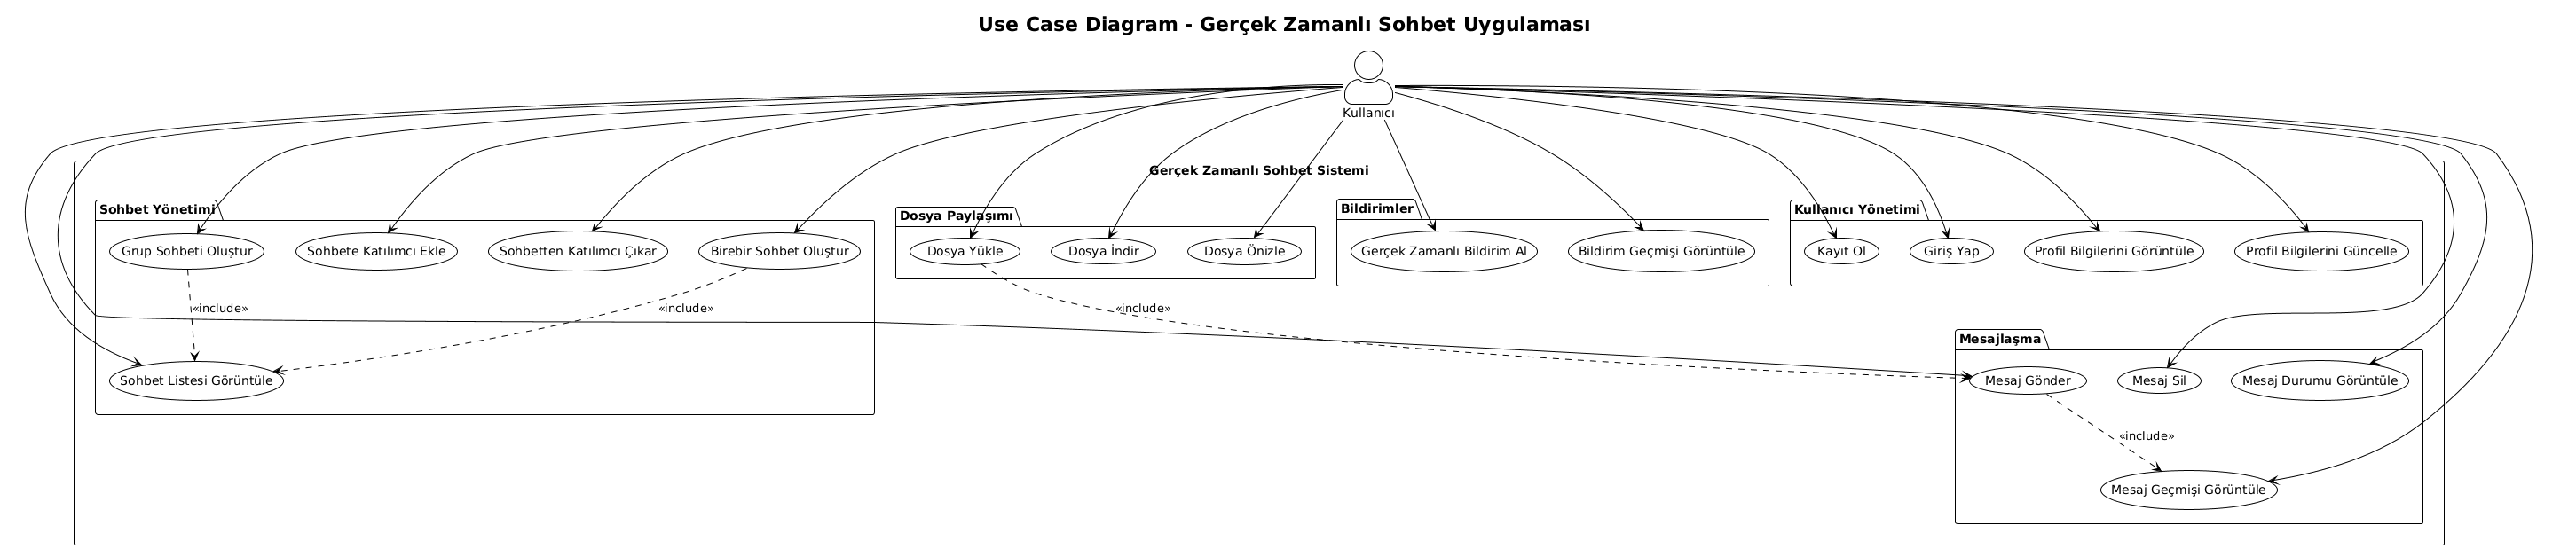
\includegraphics[width=\textwidth]{use-case.png}
    \caption{Use Case Diagram}
    \label{fig:use-case}
\end{figure}

\textbf{Aktörler:}
\begin{itemize}
    \item Authenticated User (Kimlik Doğrulanmış Kullanıcı)
\end{itemize}

\textbf{Ana Use Case'ler:}
\begin{enumerate}
    \item Kayıt Ol
    \item Giriş Yap
    \item Profil Yönetimi
    \item Birebir Sohbet Oluştur
    \item Grup Sohbeti Oluştur
    \item Sohbet Listesi Görüntüle
    \item Mesaj Gönder
    \item Mesaj Geçmişi Görüntüle
    \item Mesaj Sil
    \item Dosya Yükle
    \item Dosya İndir
    \item Bildirim Al
\end{enumerate}

\section{Domain Model (Etki Alanı Modeli)}
Domain model, sistemin temel iş varlıklarını (entities) ve aralarındaki ilişkileri gösterir.

\begin{figure}[H]
    \centering
    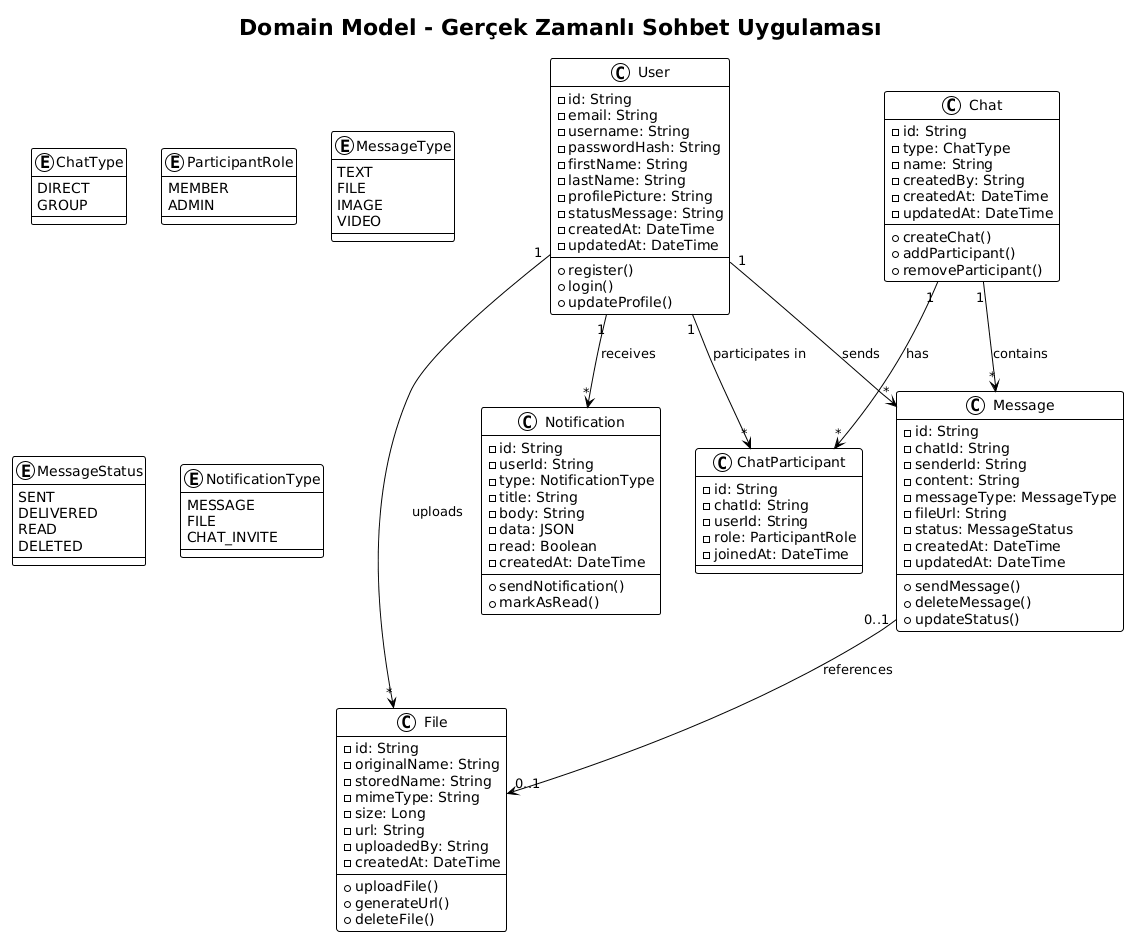
\includegraphics[width=\textwidth]{domain-model.png}
    \caption{Domain Model Diagram}
    \label{fig:domain-model}
\end{figure}

\textbf{Ana Varlıklar:}
\begin{itemize}
    \item \textbf{User (Kullanıcı):} id, email, username, passwordHash, firstName, lastName, profilePicture, statusMessage, createdAt, updatedAt
    \item \textbf{Chat (Sohbet):} id, type (DIRECT, GROUP), name, createdBy, createdAt, updatedAt
    \item \textbf{ChatParticipant (Sohbet Katılımcısı):} id, chatId, userId, role (MEMBER, ADMIN), joinedAt
    \item \textbf{Message (Mesaj):} id, chatId, senderId, content, messageType (TEXT, FILE, IMAGE, VIDEO), fileUrl, status (SENT, DELIVERED, READ, DELETED), createdAt, updatedAt
    \item \textbf{File (Dosya):} id, originalName, storedName, mimeType, size, url, uploadedBy, createdAt
    \item \textbf{Notification (Bildirim):} id, userId, type (MESSAGE, FILE, CHAT_INVITE), title, body, data, read, createdAt
\end{itemize}

\textbf{Varlık İlişkileri:}
\begin{itemize}
    \item User 1..* ChatParticipant
    \item Chat 1..* ChatParticipant
    \item Chat 1..* Message
    \item User 1..* Message
    \item User 1..* File
    \item User 1..* Notification
\end{itemize}

\section{Activity Diagram}
Activity diagram, sistem içindeki iş akışlarını gösterir.

\begin{figure}[H]
    \centering
    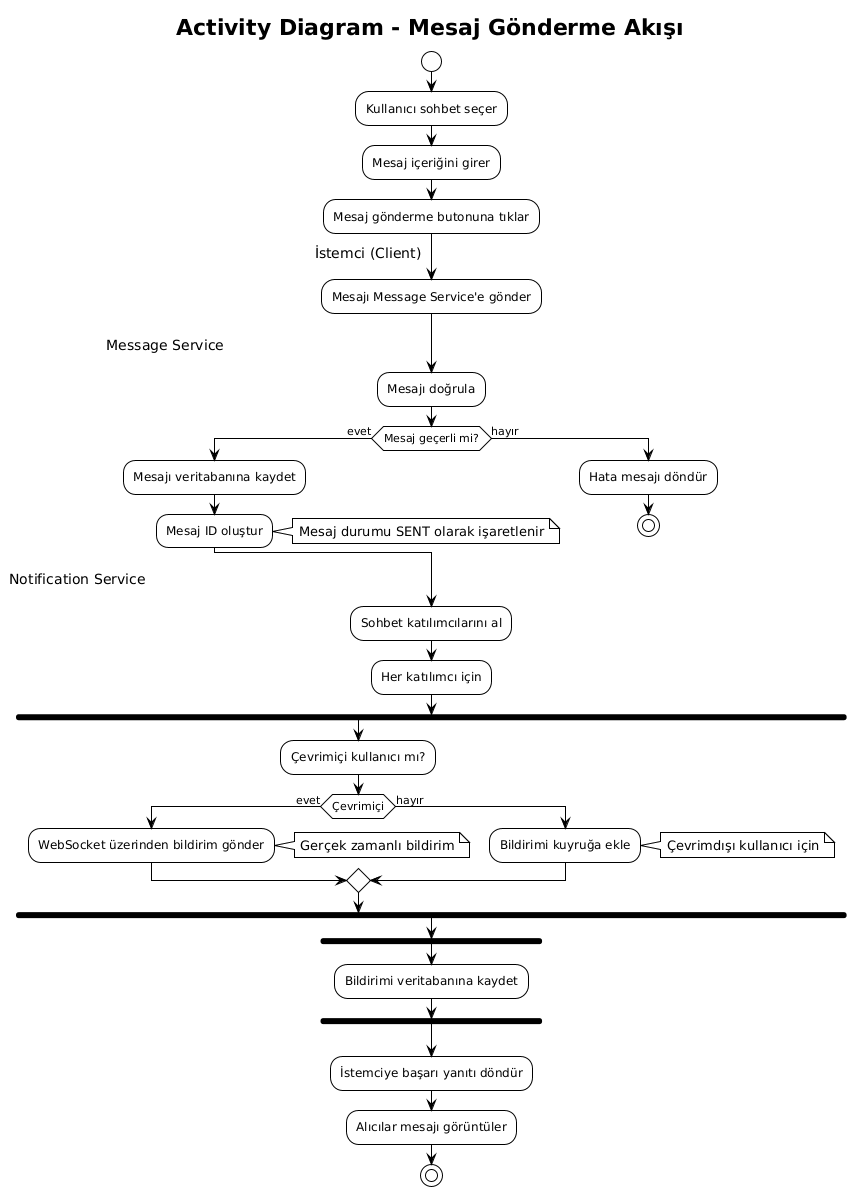
\includegraphics[width=0.8\textwidth]{activity-diagram.png}
    \caption{Mesaj Gönderme Activity Diagram}
    \label{fig:activity-message}
\end{figure}

\begin{figure}[H]
    \centering
    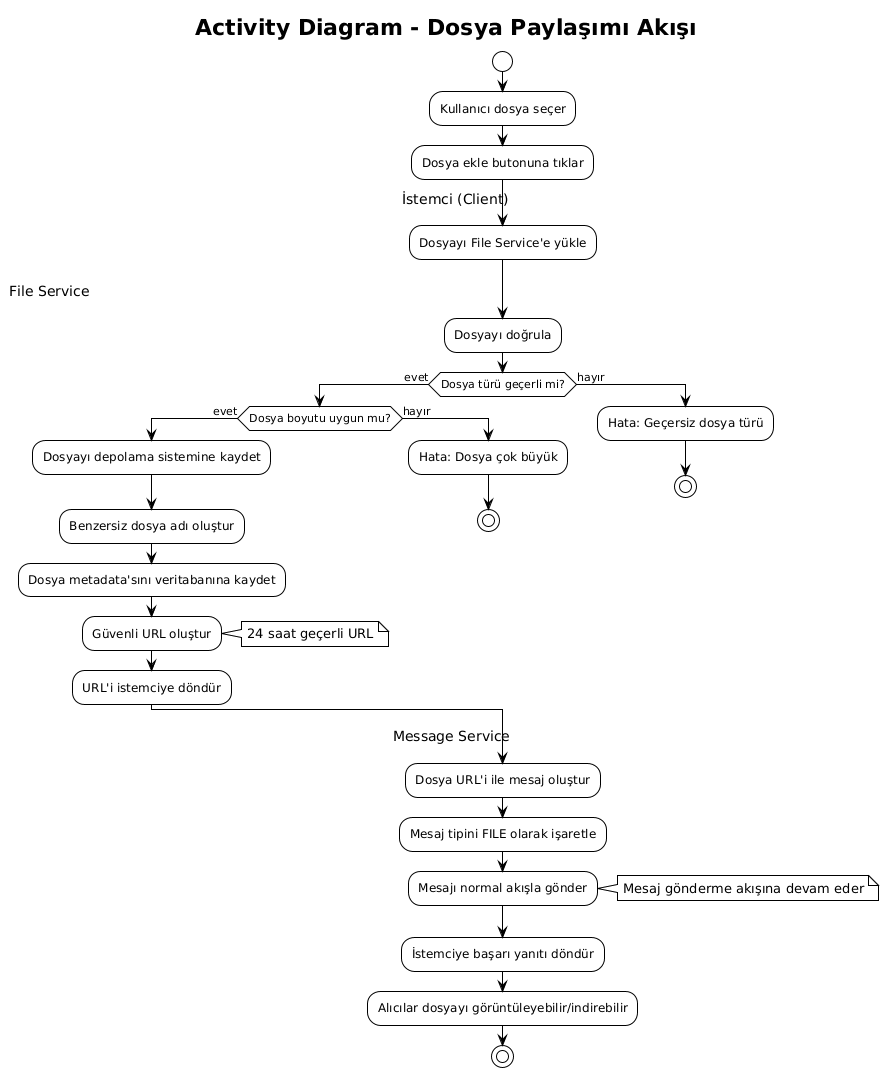
\includegraphics[width=0.8\textwidth]{activity-diagram-file-upload.png}
    \caption{Dosya Yükleme Activity Diagram}
    \label{fig:activity-file}
\end{figure}

Aşağıdaki ana akışlar modellenmiştir:
\begin{enumerate}
    \item \textbf{Mesaj Gönderme Akışı:} Mesaj gönderme sürecini gösterir.
    \item \textbf{Dosya Paylaşımı Akışı:} Dosya yükleme ve paylaşma sürecini gösterir.
\end{enumerate}

Her activity diagram, sürecin adımlarını, karar noktalarını ve paralel aktiviteleri gösterir.

\chapter{Tasarım Modeli}

\section{Genel Bakış}
Tasarım modeli, sistemin teknik mimarisini ve bileşenlerini detaylandırır. Bu model, mikroservis mimarisine dayalı sistemin yapısal tasarımını ve servisler arası etkileşimleri tanımlar.

\section{Component Diagram (Bileşen Diyagramı)}
Component diagram, sistemin yazılım bileşenlerini ve aralarındaki bağımlılıkları gösterir.

\begin{figure}[H]
    \centering
    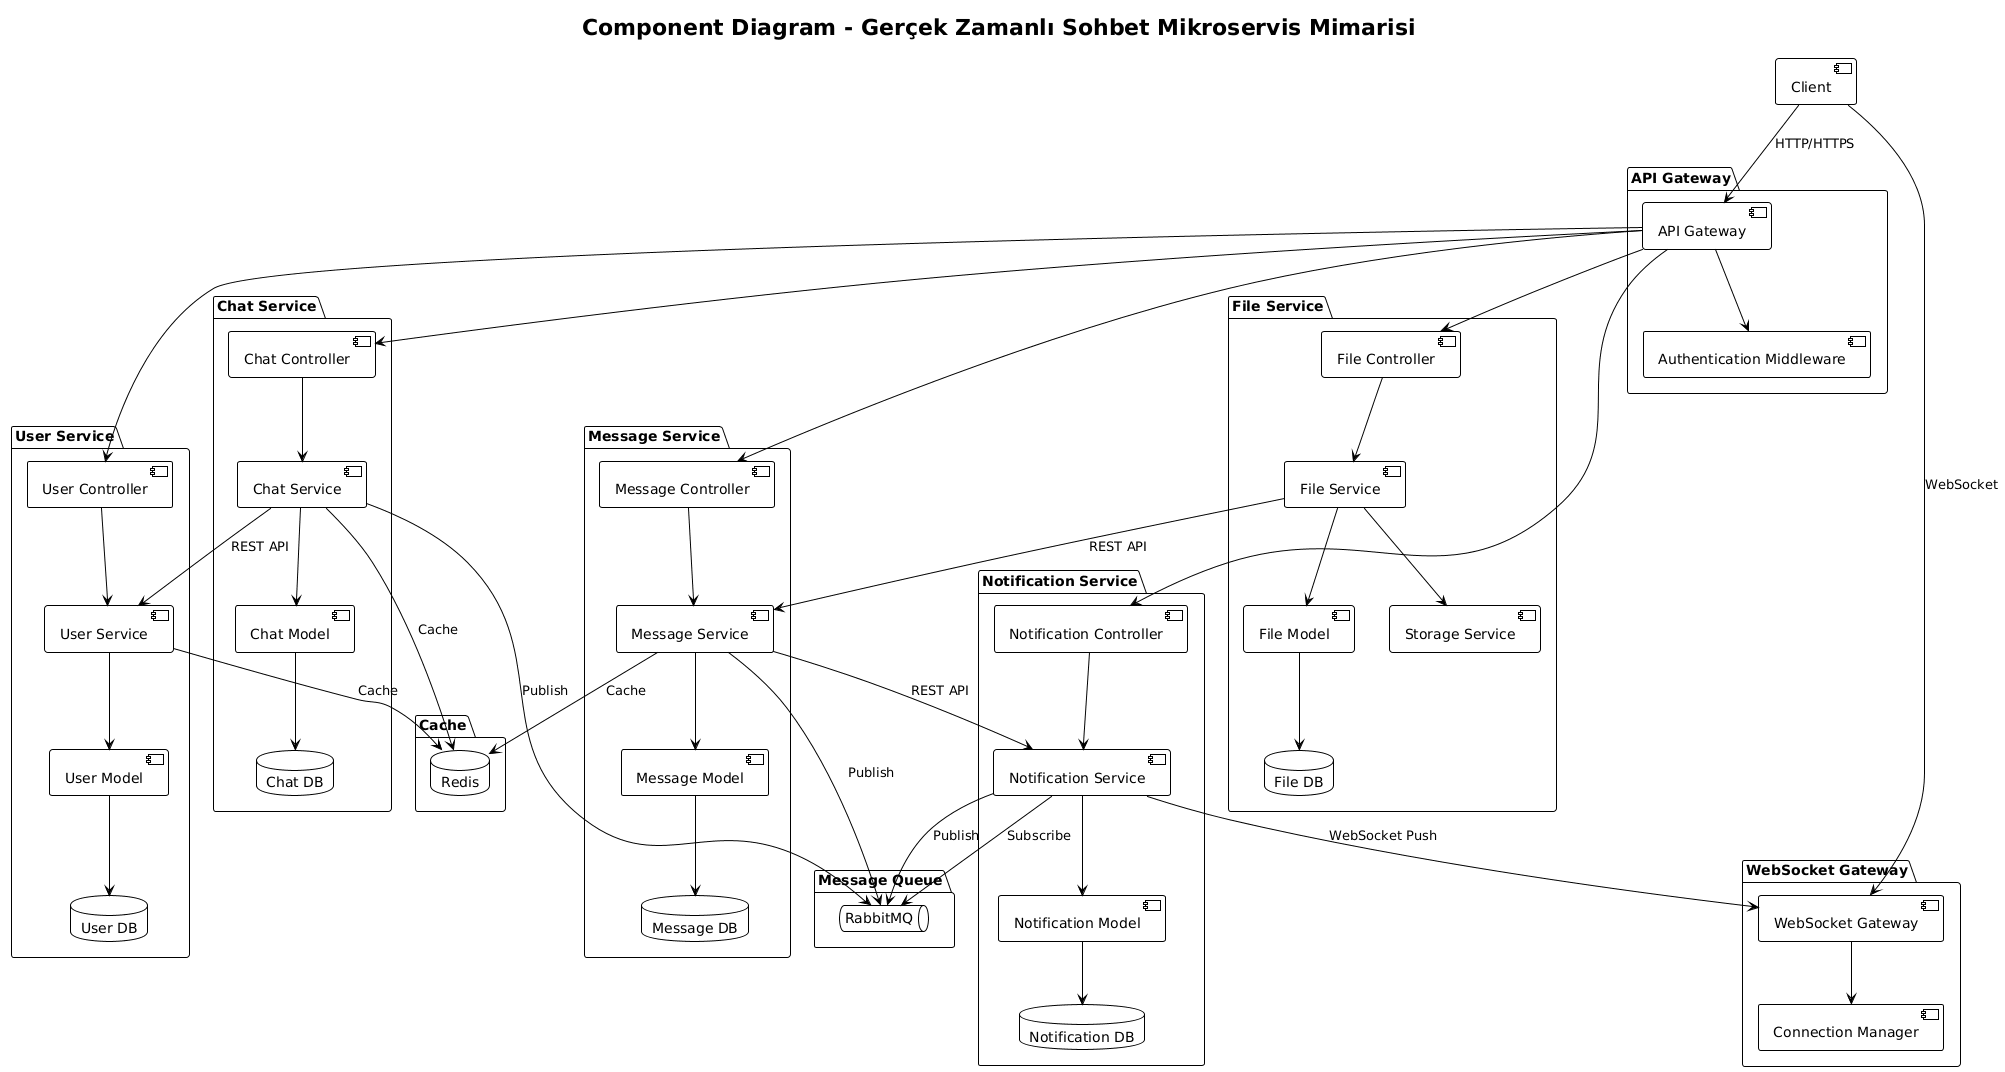
\includegraphics[width=\textwidth]{component-diagram.png}
    \caption{Component Diagram}
    \label{fig:component-diagram}
\end{figure}

\textbf{Mikroservisler:}
\begin{enumerate}
    \item User Service
    \item Chat Service
    \item Message Service
    \item Notification Service
    \item File Service
\end{enumerate}

\textbf{Altyapı Bileşenleri:}
\begin{itemize}
    \item API Gateway
    \item WebSocket Gateway
    \item Message Queue (RabbitMQ)
    \item Cache (Redis)
    \item Databases (MongoDB/PostgreSQL)
\end{itemize}

Her servis bağımsız bir bileşen olarak modellenmiş ve kendi veritabanına sahiptir. Servisler arası iletişim REST API ve message queue üzerinden gerçekleşir.

\section{Sequence Diagram (Sıralama Diyagramı)}
Sequence diagram, servisler arasındaki mesajlaşma akışını zaman sırasına göre gösterir.

\begin{figure}[H]
    \centering
    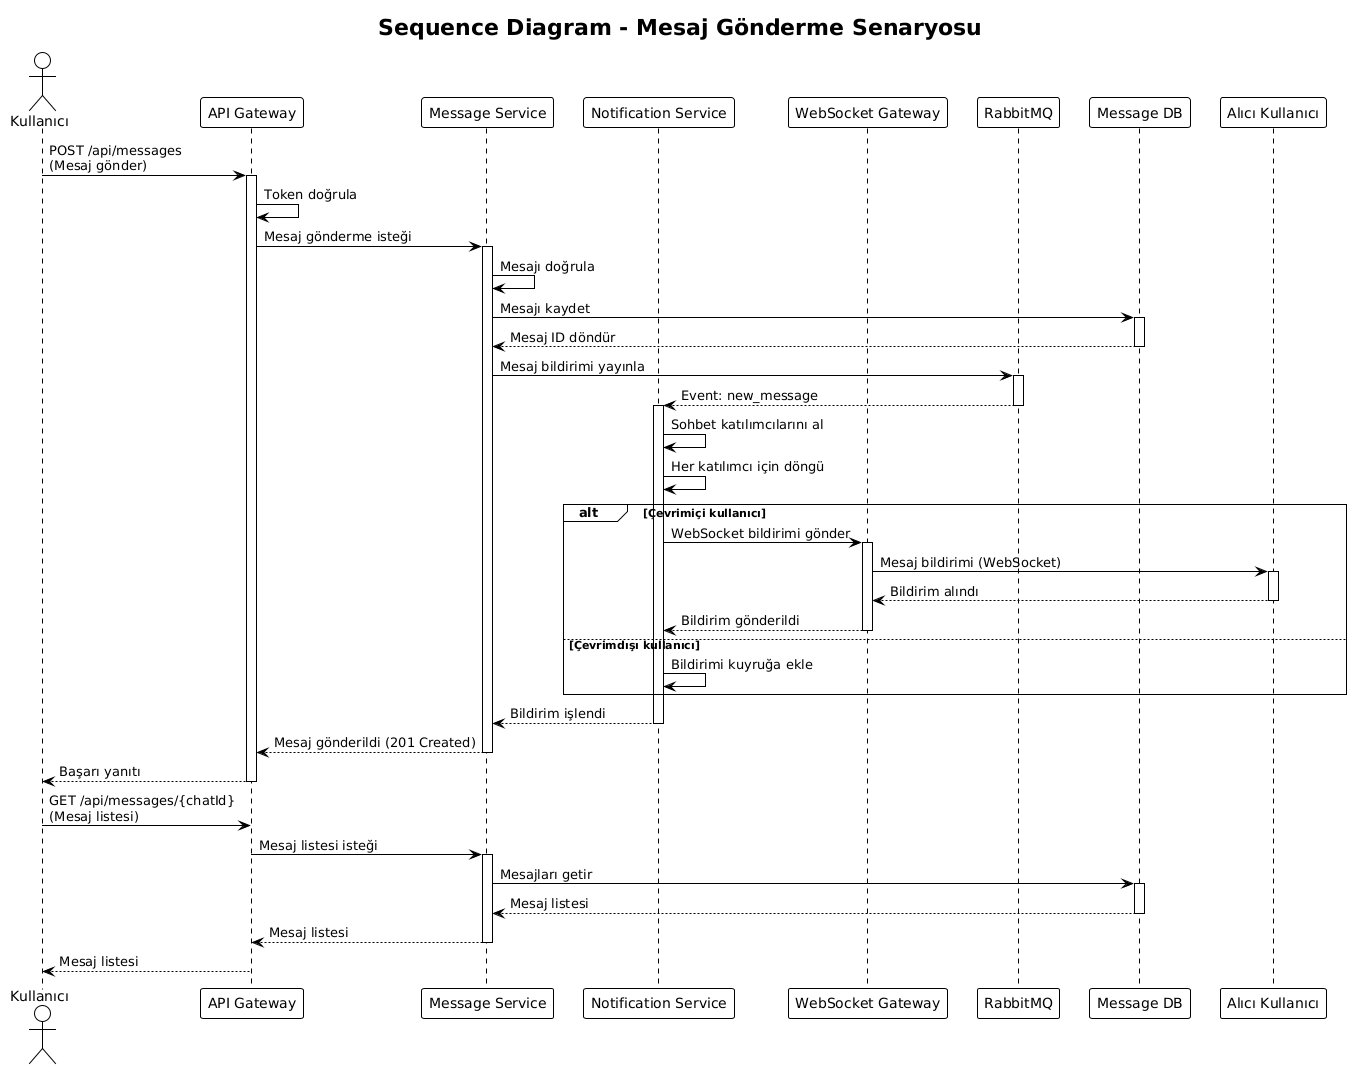
\includegraphics[width=\textwidth]{sequence-diagram.png}
    \caption{Mesaj Gönderme Sequence Diagram}
    \label{fig:sequence-message}
\end{figure}

\begin{figure}[H]
    \centering
    \includegraphics[width=\textwidth]{sequence-diagram-file-upload.png}
    \caption{Dosya Yükleme Sequence Diagram}
    \label{fig:sequence-file}
\end{figure}

Aşağıdaki kritik senaryolar modellenmiştir:
\begin{enumerate}
    \item \textbf{Mesaj Gönderme Senaryosu:} Client $\rightarrow$ API Gateway $\rightarrow$ Message Service $\rightarrow$ Notification Service $\rightarrow$ WebSocket Gateway $\rightarrow$ Client
    \item \textbf{Dosya Yükleme Senaryosu:} Client $\rightarrow$ API Gateway $\rightarrow$ File Service $\rightarrow$ Message Service
\end{enumerate}

\section{Class Diagram (Sınıf Diyagramı)}
Class diagram, her mikroservisin iç yapısını ve sınıf ilişkilerini gösterir.

\begin{figure}[H]
    \centering
    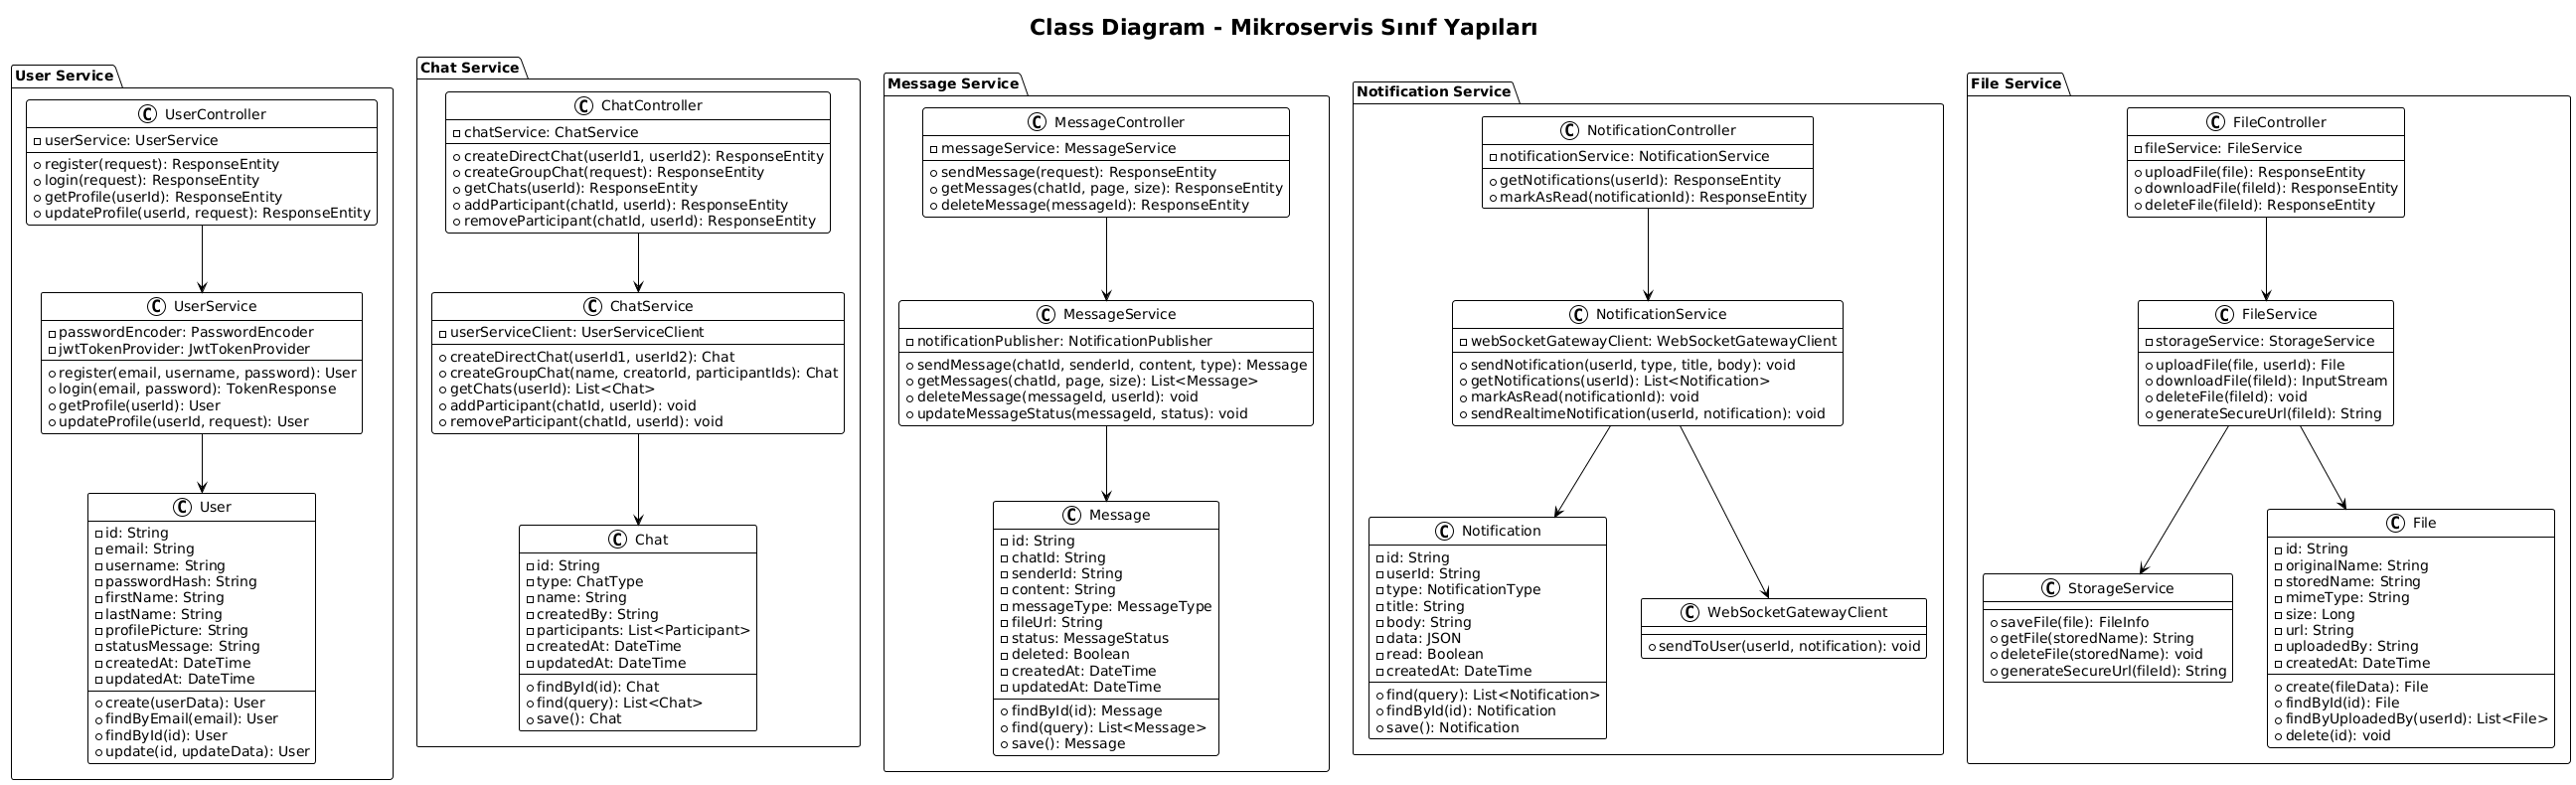
\includegraphics[width=\textwidth]{class-diagram.png}
    \caption{Class Diagram}
    \label{fig:class-diagram}
\end{figure}

Her servis için ana sınıflar:

\textbf{User Service Sınıfları:}
\begin{itemize}
    \item UserController
    \item UserService
    \item User (Model/Entity)
\end{itemize}

\textbf{Chat Service Sınıfları:}
\begin{itemize}
    \item ChatController
    \item ChatService
    \item Chat (Model/Entity)
\end{itemize}

\textbf{Message Service Sınıfları:}
\begin{itemize}
    \item MessageController
    \item MessageService
    \item Message (Model/Entity)
\end{itemize}

\textbf{Notification Service Sınıfları:}
\begin{itemize}
    \item NotificationController
    \item NotificationService
    \item Notification (Model/Entity)
    \item WebSocketGatewayClient
\end{itemize}

\textbf{File Service Sınıfları:}
\begin{itemize}
    \item FileController
    \item FileService
    \item File (Model/Entity)
    \item StorageService
\end{itemize}

\textit{Not: Her serviste veri erişimi için ayrı bir Repository katmanı yerine, Model sınıfları direkt olarak Service katmanından kullanılmaktadır. Bu yaklaşım, basitlik ve performans açısından tercih edilmiştir.}

\section{Deployment Diagram (Dağıtım Diyagramı)}
Deployment diagram, sistemin fiziksel dağıtımını ve altyapı bileşenlerini gösterir.

\begin{figure}[H]
    \centering
    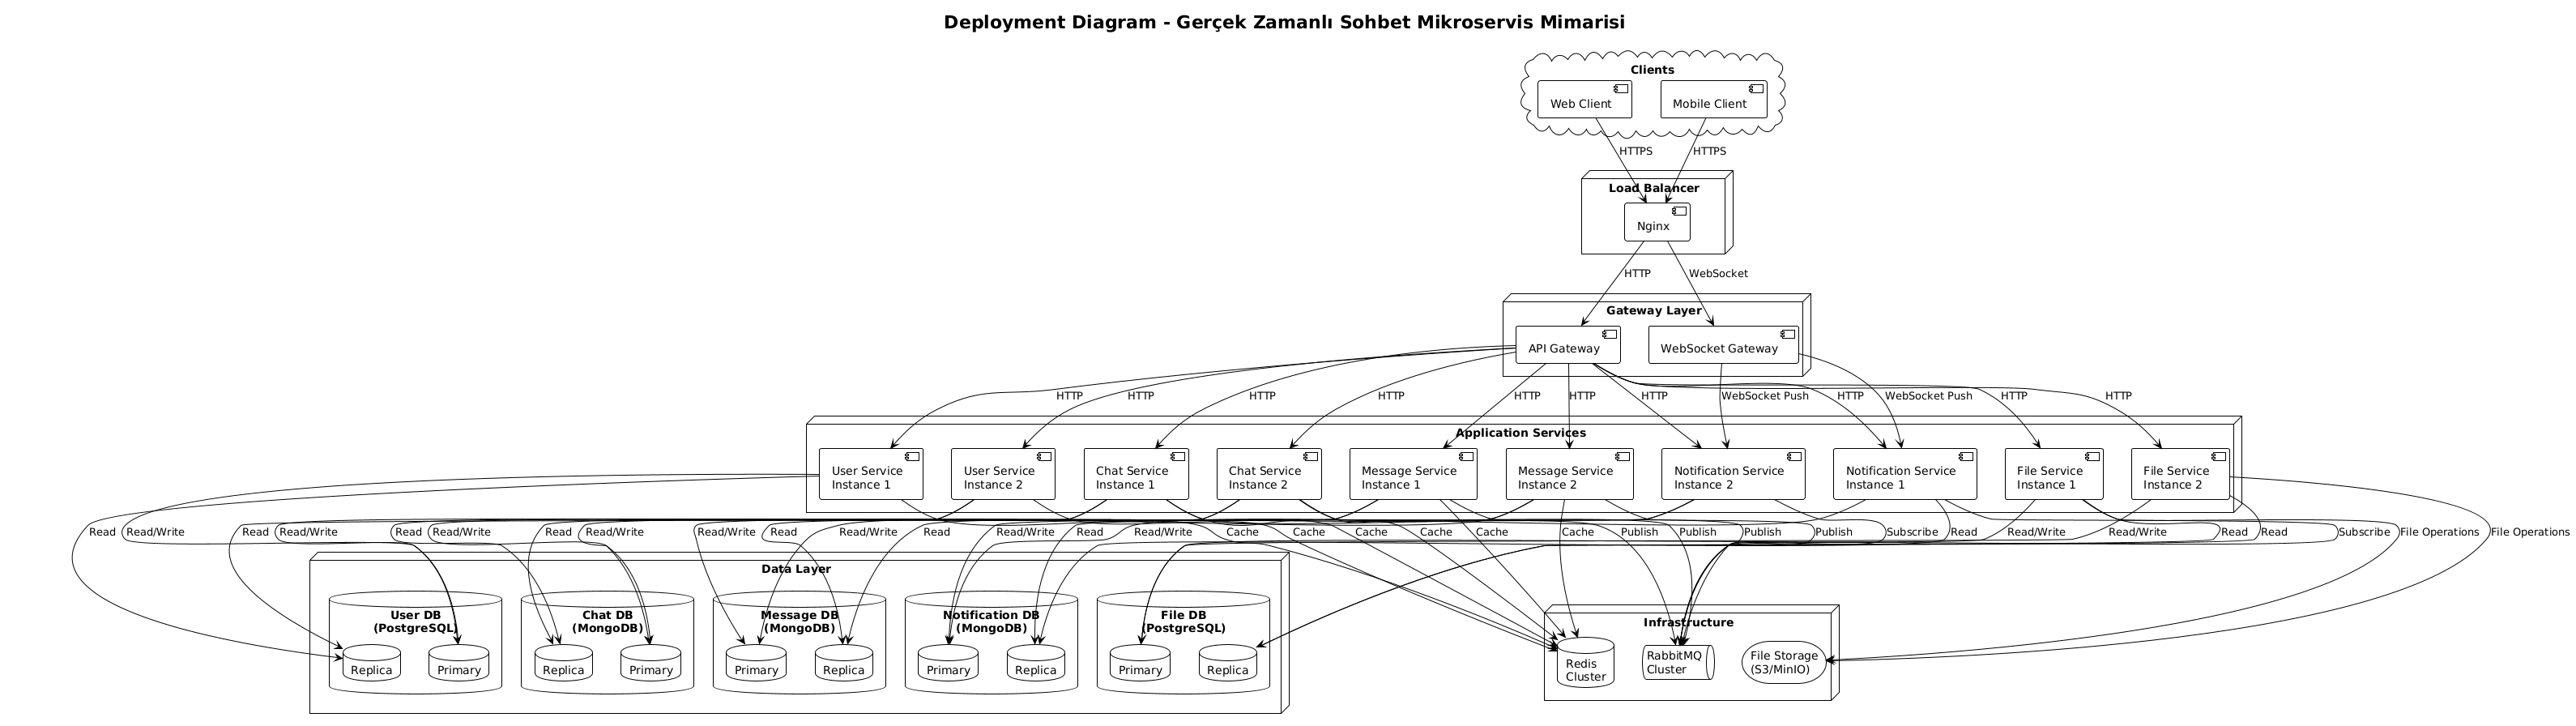
\includegraphics[width=\textwidth]{deployment-diagram.png}
    \caption{Deployment Diagram}
    \label{fig:deployment-diagram}
\end{figure}

Sistem aşağıdaki düğümlerde (nodes) çalışır:

\textbf{Container Düğümleri:}
\begin{itemize}
    \item API Gateway Container
    \item WebSocket Gateway Container
    \item 5 Mikroservis Container'ları
\end{itemize}

\textbf{Altyapı Düğümleri:}
\begin{itemize}
    \item Message Queue Node (RabbitMQ)
    \item Cache Node (Redis)
    \item Database Nodes (MongoDB/PostgreSQL)
    \item Storage Node (File Storage)
\end{itemize}

Her düğüm, containerization (Docker) ile yönetilir ve orchestration (Docker Compose) ile koordine edilir.

\section{Tasarım Prensipleri}

\subsection{Mikroservis Prensipleri}
\begin{itemize}
    \item \textbf{Bağımsız Dağıtılabilirlik:} Her servis bağımsız olarak dağıtılabilir.
    \item \textbf{Tek Sorumluluk:} Her servis belirli bir iş alanından sorumludur.
    \item \textbf{Veritabanı Ayrımı:} Her servis kendi veritabanına sahiptir.
    \item \textbf{API Tabanlı İletişim:} Servisler REST API ve message queue ile iletişim kurar.
\end{itemize}

\subsection{Tasarım Desenleri}
\begin{itemize}
    \item \textbf{API Gateway Pattern:} Tüm dış istekler API Gateway üzerinden yönlendirilir.
    \item \textbf{Event-Driven Architecture:} Asenkron işlemler için message queue kullanılır.
    \item \textbf{Circuit Breaker:} Servis hatalarına karşı dayanıklılık sağlar.
\end{itemize}

\chapter{Mimari Tasarım}

\section{Genel Mimari Yaklaşım}
Sistem, mikroservis mimarisine dayalı olarak tasarlanmıştır. Bu mimari, sistemin ölçeklenebilirliğini, dayanıklılığını ve bakım kolaylığını artırmak için tercih edilmiştir. Her mikroservis, bağımsız olarak geliştirilebilir, test edilebilir, dağıtılabilir ve ölçeklendirilebilir.

\subsection{Mimari Prensipler}
\begin{itemize}
    \item \textbf{Bağımsız Dağıtılabilirlik:} Her servis bağımsız olarak dağıtılabilir.
    \item \textbf{Tek Sorumluluk:} Her servis belirli bir iş alanından (domain) sorumludur.
    \item \textbf{Veritabanı Ayrımı:} Her servis kendi veritabanına sahiptir (Database per Service).
    \item \textbf{API Tabanlı İletişim:} Servisler REST API ve message queue ile iletişim kurar.
    \item \textbf{Hata Toleransı:} Bir servisin çökmesi tüm sistemi etkilemez.
\end{itemize}

\section{Mikroservisler ve Sorumlulukları}

\subsection{User Service}
\textbf{Sorumluluklar:}
\begin{itemize}
    \item Kullanıcı kaydı ve doğrulama
    \item Kullanıcı girişi ve kimlik doğrulama (JWT token oluşturma)
    \item Profil yönetimi (görüntüleme, güncelleme)
    \item Kullanıcı bilgilerini diğer servislere sağlama
\end{itemize}

\textbf{Teknolojiler:}
\begin{itemize}
    \item Veritabanı: PostgreSQL (Kullanıcı bilgileri)
    \item Bağımlılıklar: Redis (Cache)
\end{itemize}

\subsection{Chat Service}
\textbf{Sorumluluklar:}
\begin{itemize}
    \item Birebir ve grup sohbeti oluşturma
    \item Sohbet listesi yönetimi
    \item Sohbet katılımcı yönetimi (ekleme, çıkarma)
    \item Sohbet metadata yönetimi
\end{itemize}

\textbf{Teknolojiler:}
\begin{itemize}
    \item Veritabanı: MongoDB (Sohbet bilgileri ve katılımcıları)
    \item Bağımlılıklar: User Service, RabbitMQ, Redis
\end{itemize}

\subsection{Message Service}
\textbf{Sorumluluklar:}
\begin{itemize}
    \item Mesaj gönderme ve depolama
    \item Mesaj geçmişi sorgulama (pagination)
    \item Mesaj silme (soft delete)
    \item Mesaj durumu yönetimi (sent, delivered, read, deleted)
\end{itemize}

\textbf{Teknolojiler:}
\begin{itemize}
    \item Veritabanı: MongoDB (Mesaj bilgileri)
    \item Bağımlılıklar: RabbitMQ, Redis, User Service
\end{itemize}

\subsection{Notification Service}
\textbf{Sorumluluklar:}
\begin{itemize}
    \item Gerçek zamanlı bildirim gönderme (WebSocket)
    \item Bildirim kuyruğu yönetimi (çevrimdışı kullanıcılar için)
    \item Bildirim geçmişi saklama
    \item Bildirim durumu yönetimi (okundu/okunmadı)
\end{itemize}

\textbf{Teknolojiler:}
\begin{itemize}
    \item Veritabanı: MongoDB (Bildirim bilgileri)
    \item Bağımlılıklar: RabbitMQ, WebSocket Gateway, Redis, Chat Service
\end{itemize}

\subsection{File Service}
\textbf{Sorumluluklar:}
\begin{itemize}
    \item Dosya yükleme ve depolama
    \item Dosya indirme ve URL oluşturma
    \item Dosya türü ve boyut kontrolü
    \item Güvenli dosya erişimi
\end{itemize}

\textbf{Teknolojiler:}
\begin{itemize}
    \item Veritabanı: PostgreSQL (Dosya metadata)
    \item Bağımlılıklar: Storage Service (Local file system)
\end{itemize}

\section{Altyapı Bileşenleri}

\subsection{API Gateway}
Tüm dış HTTP isteklerini yönlendirir, kimlik doğrulama, yetkilendirme ve rate limiting (60 request/dakika/IP) işlemlerini gerçekleştirir. Node.js (Express) ve http-proxy-middleware kullanılmıştır.

\subsection{WebSocket Gateway}
Gerçek zamanlı mesaj iletimi ve bağlantı yönetimini sağlar. Kullanıcı bağlantı durumu Redis üzerinde takip edilir. Node.js ve Socket.io kullanılmıştır.

\subsection{Message Queue (RabbitMQ)}
Servisler arası asenkron iletişimi ve event-driven mimariyi destekler. `chat.exchange` ve `message.exchange` üzerinden bildirimler Notification Service'e iletilir.

\subsection{Cache (Redis)}
Sık kullanılan verilerin (sohbet listesi, son mesajlar) cache'lenmesi ve kullanıcı bağlantı durumunun takibi için kullanılır.

\subsection{Veritabanları}
Database per Service stratejisi uygulanmıştır:
\begin{itemize}
    \item \textbf{PostgreSQL:} User Service ve File Service (İlişkisel veriler)
    \item \textbf{MongoDB:} Chat Service, Message Service ve Notification Service (Doküman tabanlı, yüksek yazma hızı gerektiren veriler)
\end{itemize}

\section{Servisler Arası İletişim Desenleri}

\subsection{Senkron İletişim (REST API)}
Anında yanıt gerektiren işlemler için kullanılır (Örn: Chat Service $\rightarrow$ User Service). Güvenlik için JWT ve servis token'ları kullanılır.

\subsection{Asenkron İletişim (Message Queue)}
Event-driven işlemler ve loose coupling için kullanılır (Örn: Message Service $\rightarrow$ RabbitMQ $\rightarrow$ Notification Service).

\subsection{Gerçek Zamanlı İletişim (WebSocket)}
Anında bildirim ve çift yönlü iletişim için kullanılır (Örn: Notification Service $\rightarrow$ WebSocket Gateway $\rightarrow$ Client).

\section{Teknoloji Stack}

\begin{itemize}
    \item \textbf{Backend:} Node.js, Express.js
    \item \textbf{Frontend:} React 19, TypeScript, Vite, Tailwind CSS, Radix UI
    \item \textbf{Veritabanı:} PostgreSQL 15, MongoDB 7
    \item \textbf{Cache \& Queue:} Redis 7, RabbitMQ 3
    \item \textbf{Altyapı:} Docker, Docker Compose, ELK Stack (Logging)
\end{itemize}

\section{Güvenlik Mimarisi}
\begin{itemize}
    \item \textbf{Kimlik Doğrulama:} JWT Token
    \item \textbf{Veri Güvenliği:} HTTPS, Bcrypt (Şifre hashleme)
    \item \textbf{Kontroller:} Rate Limiting, SQL Injection Koruması, XSS Koruması
\end{itemize}

\section{Ölçeklenebilirlik Stratejisi}
\begin{itemize}
    \item \textbf{Yatay Ölçeklenebilirlik:} Stateless servisler, Load Balancer
    \item \textbf{Veritabanı:} Read Replicas, Sharding
    \item \textbf{WebSocket:} Redis adapter ile çoklu instance desteği
\end{itemize}

\chapter{Değerlendirme ve Tartışma}

\section{Tasarımın Güçlü Yönleri}

\subsection{Mikroservis Mimarisi Avantajları}
\textbf{Bağımsız Geliştirme ve Dağıtım:} Her mikroservis bağımsız olarak geliştirilebilir ve dağıtılabilir. Farklı takımlar farklı servisler üzerinde paralel çalışabilir ve servis güncellemeleri diğer servisleri etkilemez.

\textbf{Teknoloji Çeşitliliği:} Her servis için en uygun teknoloji seçilebilir. Bu projede ilişkisel veriler için PostgreSQL, yüksek yazma hızı gerektiren doküman bazlı veriler için MongoDB kullanılmıştır.

\textbf{Ölçeklenebilirlik:} Her servis ihtiyaç duyduğu kadar ölçeklendirilebilir. Yüksek trafik alan servisler (Message Service, Notification Service) daha fazla kaynak alabilir.

\textbf{Hata İzolasyonu:} Bir servisin çökmesi diğer servisleri etkilemez, sistem genel olarak çalışmaya devam eder.

\subsection{Diğer Güçlü Yönler}
\begin{itemize}
    \item \textbf{Database per Service:} Servisler arası veri bağımlılığını ortadan kaldırır.
    \item \textbf{Event-Driven Architecture:} Loose coupling ve yüksek performans sağlar.
    \item \textbf{API Gateway:} Güvenlik ve yönlendirmeyi merkezi olarak yönetir.
    \item \textbf{WebSocket Gateway:} Gerçek zamanlı iletişimi optimize eder.
\end{itemize}

\section{Zayıf Yönler ve Zorluklar}

\subsection{Servisler Arası Veri Tutarlılığı}
Database per Service stratejisi nedeniyle distributed transaction kullanılamaz. Eventual consistency kabul edilmiştir. Örneğin, mesaj gönderildiğinde bildirim asenkron olarak gönderilir; bildirim servisi geçici olarak çökerse bildirim gecikebilir.

\textbf{Çözüm:} Message queue'da mesaj persistence, retry mekanizması ve dead letter queue kullanımı.

\subsection{Distributed System Karmaşıklığı}
Mikroservis mimarisi, monolitik yapıya göre daha karmaşıktır. Network hataları ve latency sorunları yaşanabilir.

\textbf{Çözüm:} Circuit breaker pattern, timeout mekanizmaları ve health check'ler.

\subsection{Operasyonel Karmaşıklık}
Birden fazla servisin yönetimi, loglama ve izleme zordur.

\textbf{Çözüm:} Merkezi loglama (ELK Stack), container orchestration (Docker Compose) ve monitoring araçları.

\section{İyileştirme Önerileri}

\begin{enumerate}
    \item \textbf{Service Mesh:} Istio veya Linkerd kullanılarak servisler arası iletişim, güvenlik ve gözlemlenebilirlik iyileştirilebilir.
    \item \textbf{CQRS (Command Query Responsibility Segregation):} Okuma ve yazma işlemlerinin ayrılması performans optimizasyonu sağlar.
    \item \textbf{Saga Pattern:} Distributed transaction yerine uzun süren işlemler (örn: grup oluşturma) için Saga pattern kullanılabilir.
    \item \textbf{API Versioning:} Geriye dönük uyumluluk için `/api/v1/` gibi versiyonlama stratejisi uygulanmalıdır.
    \item \textbf{Caching İyileştirmeleri:} Multi-level caching (L1: in-memory, L2: Redis) ile veritabanı yükü azaltılabilir.
    \item \textbf{Monitoring:} Prometheus ve Grafana ile kapsamlı metrik takibi ve alarm mekanizmaları kurulabilir.
\end{enumerate}

\section{Sonuç}
Gerçek zamanlı sohbet uygulaması için tasarlanan bu mikroservis mimarisi; ölçeklenebilirlik, dayanıklılık ve bakım kolaylığı sağlamaktadır. Sistem, 5 bağımsız mikroservis ve destekleyici altyapı bileşenlerinden oluşmaktadır. Her servis kendi sorumluluğunu yerine getirir ve sistem genel olarak yüksek performans ve güvenilirlik hedefler. Tasarımın getirdiği karmaşıklıklar, doğru stratejiler (Event-driven, API Gateway, Merkezi Loglama) ile yönetilmiştir.


% Kaynakça (Eğer varsa)
% \bibliographystyle{plain}
% \bibliography{references}

\end{document}
